\documentclass[24pt, a0paper, landscape]{tikzposter}
\usepackage[utf8]{inputenc}
\usepackage{graphicx}
\usepackage[labelsep=period]{caption}

\usepackage{url}
\usepackage{hyperref}
\hypersetup{
colorlinks=true,
linkcolor=blue,
filecolor=magenta,
urlcolor=cyan,
}

\title{Nirdizati Training}
\author{Stanislav Mõškovski\\{\small \textit{Supervised by Ilya Verenich, MSc}}}
\date{today}
\institute{Institute of Computer Science, University of Tartu}


\begin{document}
    \maketitle

    \begin{columns}
        \column{0.3}
        \block{Description}
        {
        Write in general what is Nirdizati Training component.
        What is the purpose of this?
        Who is it targeted at?
        }

        \block{Problems of existing solutions}
        {
        Briefly mention problems of existing solutions.
        What are their weaknesses?
        What are their shortcomings?
        }

        \block{Advantages of our solution}
        {
        Describe advantages of our solution.
        Those can be taken from thesis.
        }

        \block{Interoperability}
        {
        Write about how output of the application can be used for further
        analysis.
        Mention that model can by deployed to Nirdizati Runtime component.
        }

        \column{0.4}
        \block{User interface}
        {
        \begin{tikzfigure}[Training view of Nirdizati Training component.]
            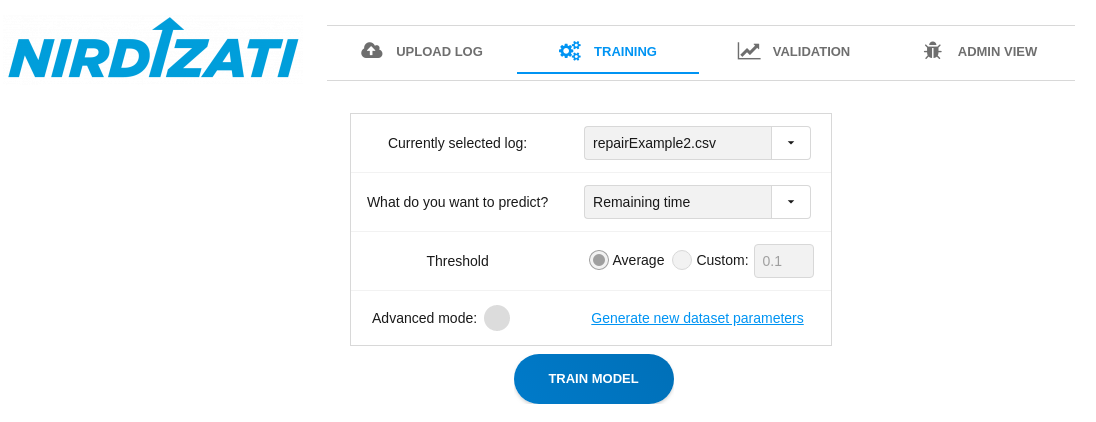
\includegraphics{figures/training.png}
        \end{tikzfigure}

        \begin{tikzfigure}[View of completed simulations, which allows sorting and grouping by various parameters.]
            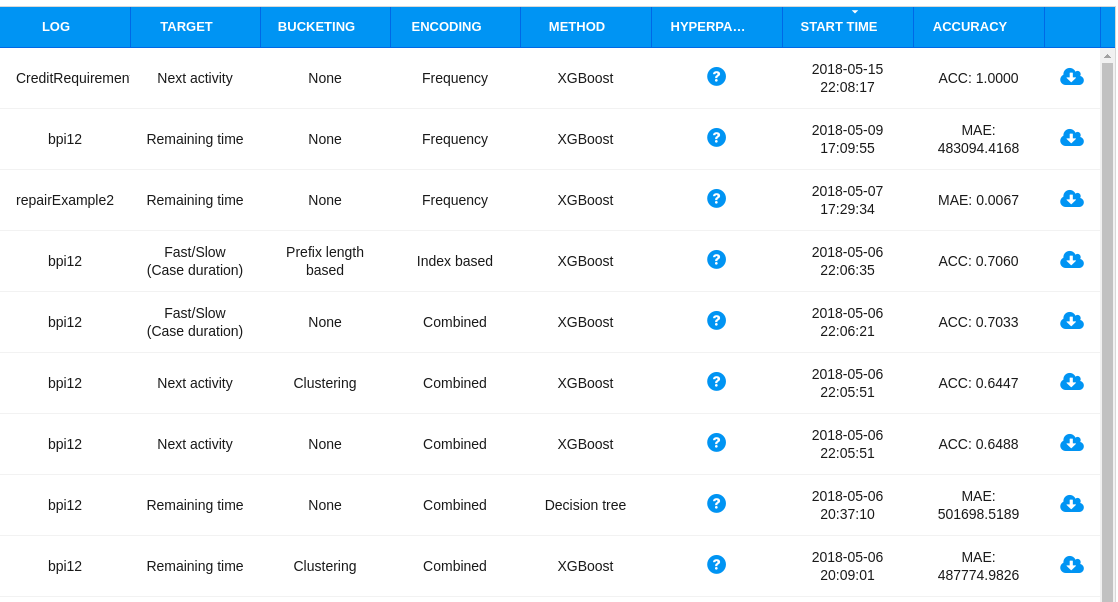
\includegraphics{figures/validation.png}
        \end{tikzfigure}

        \begin{tikzfigure}[Model evaluation view with model accuracy visualization.]
            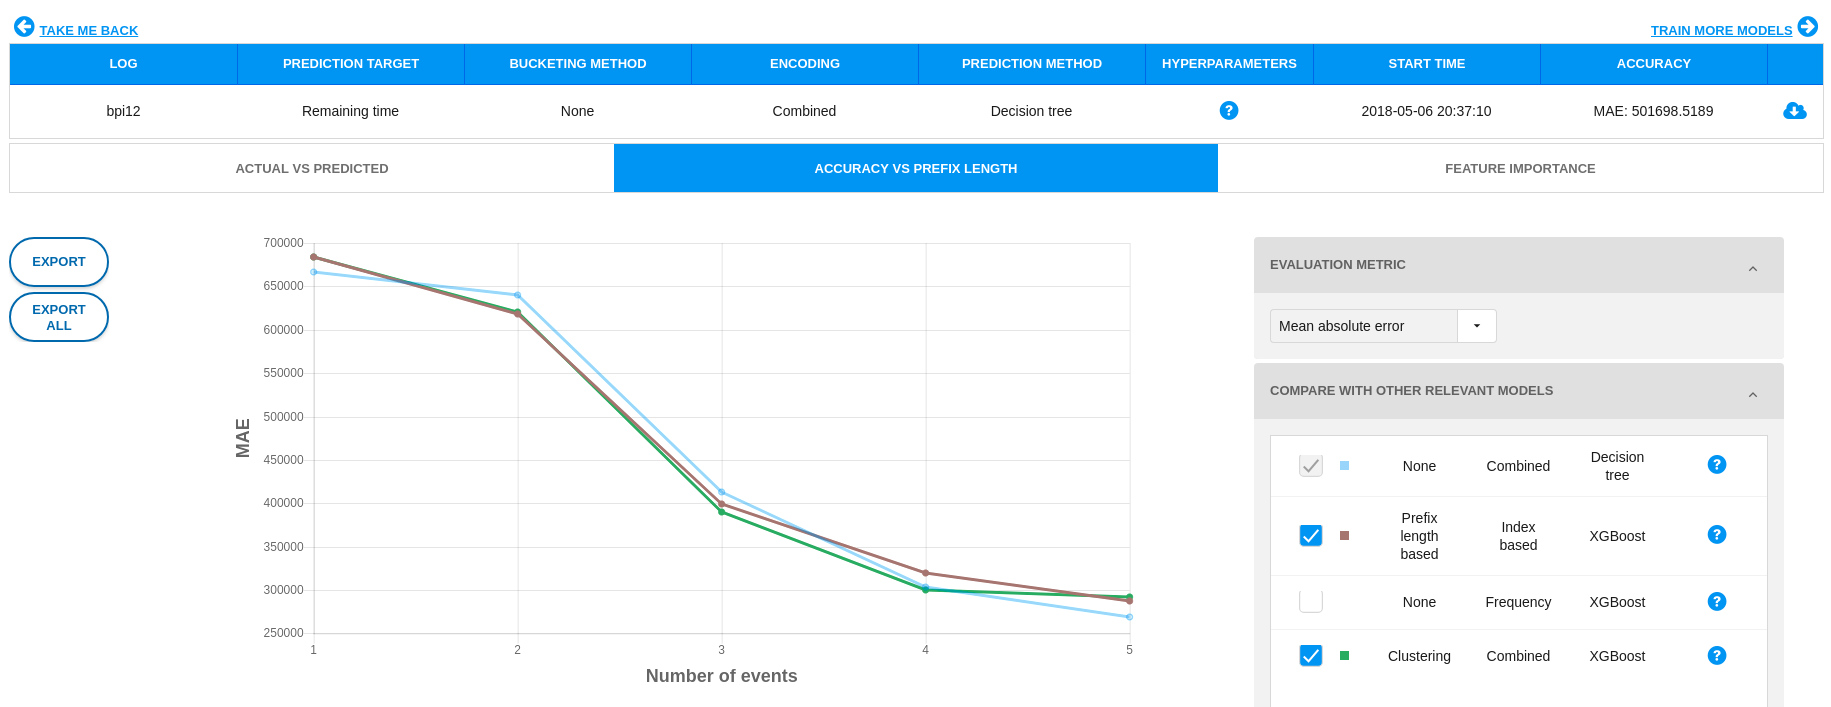
\includegraphics[scale=0.65]{figures/model_overview.png}
        \end{tikzfigure}
        }

        \column{0.3}
        \block{Technical solution}
        {
        Data flow diagram?
        Architecture diagram?
        }

        \block{Links}
        {
        \textbf{Code:} \href{https://github.com/Zukkari/nirdizati-training-ui}{\url{https://github.com/Zukkari/nirdizati-training-ui}}
        \bigbreak

        \textbf{Nirdizati:} \href{http://nirdizati.org/}{\url{http://nirdizati.org}}
        \bigbreak

        \textbf{Nirdizati Training:} \href{http://training.nirdizati.org/}{\url{http://training.nirdizati.org/}}
        \bigbreak

        \textbf{Twitter:} \href{https://twitter.com/nirdizati}{\url{https://twitter.com/nirdizati}}
        }
    \end{columns}
\end{document}